\section{Contexte}
\label{Contexte}

    À l'heure actuelle, la sécurité des systèmes est un enjeu majeur. Ainsi, de nombreuses méthodes de modélisation et d'analyse des systèmes ont été développées, dans le but d'identifier les risques et de les quantifier. C'est avec cette idée que le concept d'ADTrees\footnote{Abréviation d'\og Attack-Defense Trees \fg{}, ou \og Arbres d'Attaque et de Défense\fg{} en français.}, un formalisme permettant une représentation sous forme d'arbre des étapes d'une attaque précise contre un système, a vu le jour. L'un des logiciels permettant de modéliser ces ADTrees s'appelle ADTool.

    ADTool implémente la plupart des fonctionnalités qui peuvent être attendues de la part d'un logiciel d'édition d'ADTrees, y compris l'utilisation de paramètres tels que le coût ou le temps nécessaire pour réaliser une attaque. Mais il a été conçu comme un logiciel de modélisation avant tout, et comporte donc peu d'outils permettant d'analyser les ADTrees. 

    L'objectif de ce projet a donc été la réalisation d'un logiciel permettant de dépasser ces limites en fournissant à l'utilisateur, un expert en sécurité, des outils d'analyse des ADTrees. Ce logiciel a été nommé \glasir{} en référence à l'arbre aux feuilles d'or de la mythologie nordique~\cite{vikingCulture}, et nous avons créé son logo visible sur la \textsc{Figure} \ref{fig:glasir}. Il dispose de trois fonctionnalités principales, qui ont été détaillées dans les rapports de spécifications fonctionnelles et de conception :    
\begin{itemize}
    	\item l'{\bf Éditeur de fonctions}, qui permet à l'expert de créer de nouveaux paramètres fonctions de ceux déjà présents dans l'arbre, afin de pouvoir exprimer des compromis entre plusieurs paramètres ;
    	\item le {\bf Filtre}, qui aide l'utilisateur à ôter de l'ADTree les branches aux valuations hors d'un intervalle défini ;
    	\item l'{\bf Optimiseur}, qui sélectionne le(s) meilleur(s) chemin(s) dans l'ADTree selon un certain paramètre.
\end{itemize} 
ADTool a quant à lui été amélioré, et utilisé au sein de Glasir comme viewer d'ADTrees. 

Quatre rapports ont déjà été rédigés dans le cadre de ce projet : celui de pré-étude~\cite{pre_etude}, celui de spécifications fonctionnelles~\cite{spec_fonc}, celui de planification~\cite{planif} et celui de conception~\cite{conception}. Ils ont permis de mieux définir les objectifs du logiciel ainsi que l'organisation de son implémentation. Le but de ce rapport final est de rendre compte de la tenue des objectifs qui ont été fixés au début du projet, des méthodes mises en place pour y parvenir, ainsi que des ajustements qui ont du être mis en place afin de gérer les imprévus auquels nous avons fait face. 

Pour rendre compte de tout cela, ce rapport est composé d'une collection de documents indépendants couvrant l'ensemble de ces aspects : rectificatifs de conception, compte-rendus de tests, description des livrables, et pour finir une retrospective sur la conduite de ce projet.

    \begin{figure}[!h]
        \centering
        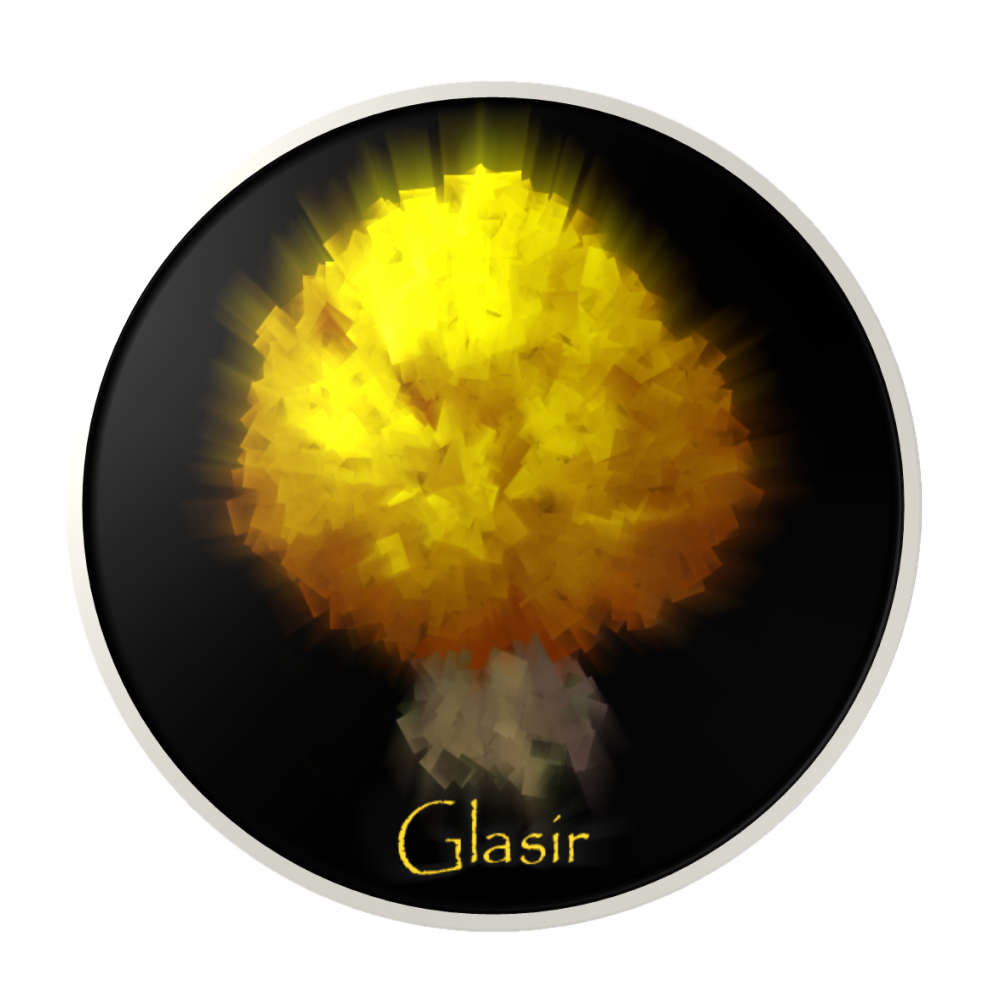
\includegraphics[height=0.5\textwidth]{figure/glasir.png}
        \caption{Logo du logiciel Glasir.}
        \label{fig:glasir}
    \end{figure}